\section{Group - Zone Equipment}\label{group---zone-equipment}

There are five main zone equipment statements that must be used to describe a block of zone equipment as shown in Figure \ref{fig:zone-equipment-syntax-map} - ``Zone Equipment Input Syntax Map'' below:

\begin{figure}[hbtp]
\centering
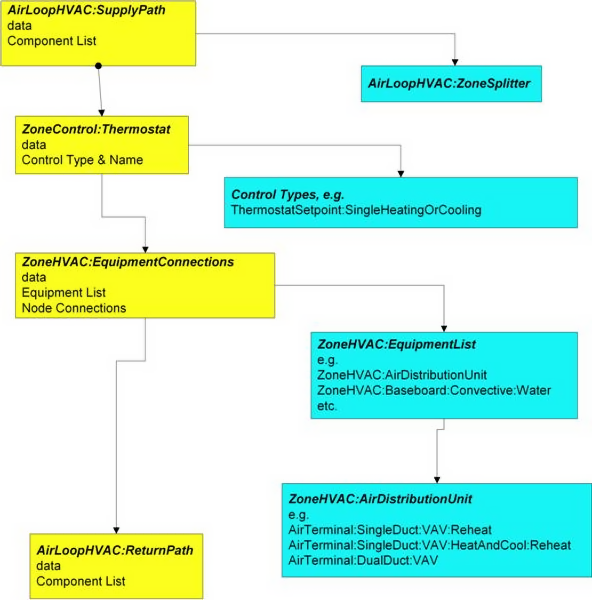
\includegraphics[width=0.9\textwidth, height=0.9\textheight, keepaspectratio=true]{media/image261.png}
\caption{Zone Equipment Input Syntax Map \protect \label{fig:zone-equipment-syntax-map}}
\end{figure}

Types of Zone equipment are listed below and shown below in figure ``Zone Equipment''.

% table 26
\begin{longtable}[c]{p{1.5in}p{4.5in}}
\caption{Available Zone Equipment Types \label{table:available-zone-equipment-types}} \tabularnewline
\toprule
Air Distribution Equipment & AirTerminal:SingleDuct:ConstantVolume:Reheat     AirTerminal:SingleDuct:ConstantVolume:NoReheat    AirTerminal:SingleDuct:VAV:Reheat    AirTerminal:SingleDuct:VAV:NoReheat    AirTerminal:SingleDuct:VAV:Reheat:VariableSpeedFan    AirTerminal:DualDuct:ConstantVolume    AirTerminal:DualDuct:VAV    Powered Induction Units (Series and Parallel) \tabularnewline
\midrule
\endfirsthead

\caption[]{Available Zone Equipment Types} \tabularnewline
\toprule
Air Distribution Equipment & AirTerminal:SingleDuct:ConstantVolume:Reheat    AirTerminal:SingleDuct:ConstantVolume:NoReheat    AirTerminal:SingleDuct:VAV:Reheat    AirTerminal:SingleDuct:VAV:NoReheat    AirTerminal:SingleDuct:VAV:Reheat:VariableSpeedFan    AirTerminal:DualDuct:ConstantVolume    AirTerminal:DualDuct:VAV    Powered Induction Units (Series and Parallel) \tabularnewline
\midrule
\endhead

Zone Forced Air Units ~ & ZoneHVAC:IdealLoadsAirSystem    ZoneHVAC:FourPipeFanCoil    ZoneHVAC:WindowAirConditioner    ZoneHVAC:RefrigerationChillerSet    Unit Ventilator/Heater    Air-to-Air Heat Pumps    Unitary Systems (heat only and heat/cool)    Furnaces (heat only and heat/cool)    Energy Recovery Ventilator:Stand Alone    CoilSystem:Cooling:DX \tabularnewline
Radiative/Convective Units & Baseboard Heaters    Low Temp Radiant Systems    High Temp Radiant System \tabularnewline
\bottomrule
\end{longtable}

\begin{figure}[hbtp]
\centering
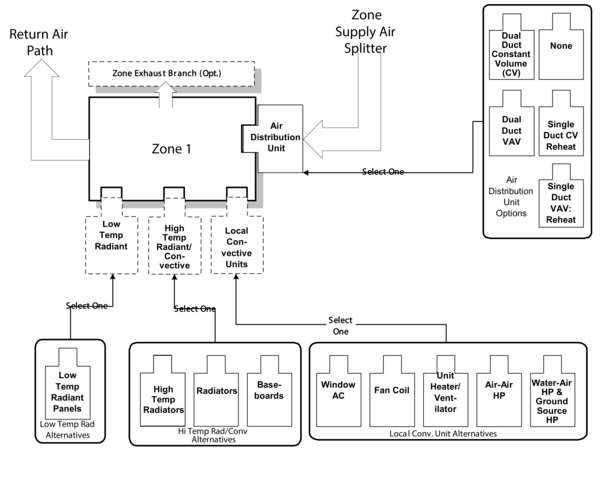
\includegraphics[width=0.8\textwidth, keepaspectratio=true]{media/image262.png}
\caption{Representative Zone Equipment \protect \label{fig:representative-zone-equipment}}
\end{figure}

The following Figure \ref{fig:air-loopzone-equipment-node-diagram} ``Air Loop/Zone Equipment Node Diagram'' illustrates the connection between the zone equipment and the air loop systems.

\begin{figure}[hbtp]
\centering
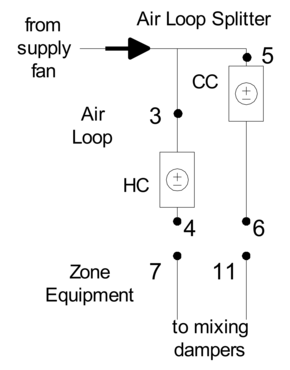
\includegraphics[width=0.4\textwidth, keepaspectratio=true]{media/image263.png}
\caption{Air Loop/Zone Equipment Node Diagram \protect \label{fig:air-loopzone-equipment-node-diagram}}
\end{figure}

Each zone served by an HVAC system must have three additional statements to complete the zone equipment specification. An \hyperref[zonehvacairdistributionunit]{ZoneHVAC:AirDistributionUnit} allows equipment typically found within the zone inlet ductwork (such as dampers, reheat coils, etc.) to be attached to the supply air stream for a particular zone. A ZoneControl statement will allow the conditions in the zone to be managed. Finally, a \hyperref[zonehvacequipmentconnections]{ZoneHVAC:EquipmentConnections} statement describes all of the pertinent information about the zone from an HVAC perspective. Each of these statements is described in more detail below.

\subsection{ZoneHVAC:AirDistributionUnit}\label{zonehvacairdistributionunit}

The ZoneHVAC:AirDistributionUnit object gives further information on what air loop equipment (air terminal units) will be serving a particular zone. The ZoneHVAC:AirDistributionUnit is the part of the system that is supplied from a common main air handler simulated in the Air Loop Simulation and includes the equipment that controls or tempers the air going to each individual zone according to the desired thermostatic control. The current options for ZoneHVAC:AirDistributionUnit terminal unit types are:

\begin{itemize}
\item
  \hyperref[airterminaldualductconstantvolume]{AirTerminal:DualDuct:ConstantVolume}
\item
  \hyperref[airterminaldualductvav]{AirTerminal:DualDuct:VAV}
\item
  \hyperref[airterminaldualductvavoutdoorair]{AirTerminal:DualDuct:VAV:OutdoorAir}
\item
  \hyperref[airterminalsingleductconstantvolumereheat]{AirTerminal:SingleDuct:ConstantVolume:Reheat}
\item
  \hyperref[airterminalsingleductvavreheat]{AirTerminal:SingleDuct:VAV:Reheat}
\item
  \hyperref[airterminalsingleductvavnoreheat]{AirTerminal:SingleDuct:VAV:NoReheat}
\item
  \hyperref[airterminalsingleductseriespiureheat]{AirTerminal:SingleDuct:SeriesPIU:Reheat}
\item
  \hyperref[airterminalsingleductparallelpiureheat]{AirTerminal:SingleDuct:ParallelPIU:Reheat}
\item
  \hyperref[airterminalsingleductconstantvolumefourpipeinduction]{AirTerminal:SingleDuct:ConstantVolume:FourPipeInduction}
\item
  \hyperref[airterminalsingleductvavreheatvariablespeedfan]{AirTerminal:SingleDuct:VAV:Reheat:VariableSpeedFan}
\item
  \hyperref[airterminalsingleductvavheatandcoolreheat]{AirTerminal:SingleDuct:VAV:HeatAndCool:Reheat}
\item
  \hyperref[airterminalsingleductvavheatandcoolnoreheat]{AirTerminal:SingleDuct:VAV:HeatAndCool:NoReheat}
\item
  \hyperref[airterminalsingleductconstantvolumecooledbeam]{AirTerminal:SingleDuct:ConstantVolume:CooledBeam}
\item
  \hyperref[airterminalsingleductuserdefined]{AirTerminal:SingleDuct:UserDefined}
\item
  \hyperref[airterminalsingleductmixer]{AirTerminal:SingleDuct:Mixer}

\end{itemize}

Connections between the air distribution unit, the supply air duct, and the zone are specified in the input syntax for the air distribution unit and the \hyperref[airloophvaczonesplitter]{AirLoopHVAC:ZoneSplitter}. The input syntax also explicitly defines an outlet identifier. This implies a connection to a zone through a \hyperref[nodelist]{NodeList} for zone inlets (see the \hyperref[zonehvacequipmentconnections]{ZoneHVAC:EquipmentConnections} statement). The air distribution unit is limited to one combined component-controller unit; because controls are normally based on the zone thermostat and can work in parallel or series in complex fashion. Since the control and the flow resolution can be complex, each air distribution unit is unique in addressing these combinations and therefore only one is allowed per zone.

The Air Distribution unit also allows the user to specify leaks in the supply air duct system. These inputs are used in the EnergyPlus Simplified Duct Leakage Model (SDLM). This model simulates a specific configuration: supply leaks to a return plenum in a commercial VAV or CV system. The system must have a constant static pressure setpoint. Within these limitations SDLM allows the user to easily evaluate the energy penalty due to duct leakage.

\subsubsection{Inputs}\label{inputs-055}

\paragraph{Field: Name}\label{field-name-053}

Unique identifying name of the air distribution unit.

\paragraph{Field: Air Distribution Unit Outlet Node Name}\label{field-air-distribution-unit-outlet-node-name}

Outlet node name for the air distribution unit to the attached zone.

\paragraph{Field: Air Terminal Object Type}\label{field-air-terminal-object-type}

Single combined component/controller unit for that attached zone. Selection of components as listed above.

\paragraph{Field: Air Terminal Name}\label{field-air-terminal-name}

The unique identifying component name.

\paragraph{Field: Nominal Upstream Leakage Fraction}\label{field-nominal-upstream-leakage-fraction}

This is the leakage upstream of the terminal unit as a fraction of the design flow rate through the unit. It is the leakage fraction at the design flow rate. It is used to calculate a leakage flow rate which is then held constant while the system air flow varies. This input is optional; the default is zero.

\paragraph{Field: Constant Downstream Leakage Fraction}\label{field-constant-downstream-leakage-fraction}

This is the leakage downstream of the terminal unit as a fraction of the current flow rate through the terminal unit. This fraction is held constant, so the leakage flow rate will vary proportinally with the supply air flow rate. This input is optional; the default is zero.

\paragraph{Field: Design Specification Air Terminal Sizing Name}\label{design-specification-air-terminal-sizing-name2}

This optional input field is the name of a \hyperref[designspecificationairterminalsizing]{DesignSpecification:AirTerminal:Sizing} object which specifies sizing adjustments to be made for the air terminal unit referenced by this object. The terminal unit is initially sized according to the inputs in the corresponding \hyperref[sizingzone]{Sizing:Zone} object. Then the adjustment factors in the \hyperref[designspecificationairterminalsizing]{DesignSpecification:AirTerminal:Sizing} object are applied. See \hyperref[designspecificationairterminalsizing]{DesignSpecification:AirTerminal:Sizing} for more details. If left blank, then no adjustments are made.

\subsubsection{Outputs}

\begin{itemize}
    \item
    HVAC,Sum,Zone Air Terminal Sensible Heating Energy {[}J{]}
    \item
    HVAC,Sum,Zone Air Terminal Sensible Cooling Energy {[}J{]}
    \item
    HVAC,Average,Zone Air Terminal Sensible Heating Rate {[}W{]}
    \item
    HVAC,Average,Zone Air Terminal Sensible Cooling Rate {[}W{]}
    \item
    HVAC,Average,Zone Air Terminal Outdoor Air Volume Flow Rate {[}m3/s{]}
\end{itemize}

\paragraph{Zone Air Terminal Sensible Heating Rate {[}W{]}}\label{zone-air-terminal-sensible-heating-rate-w}

\paragraph{Zone Air Terminal Sensible Heating Energy~ {[}J{]}}\label{zone-air-terminal-sensible-heating-energy-j}

These outputs are the sensible heating rate and energy provided to the zone by the single duct constant volume no reheat air terminal unit.

\paragraph{Zone Air Terminal Sensible Cooling Rate {[}W{]}}\label{zone-air-terminal-sensible-cooling-rate-w}

\paragraph{Zone Air Terminal Sensible Cooling Energy {[}J{]}}\label{zone-air-terminal-sensible-cooling-energy-j}

These outputs are the sensible cooling rate and energy provided to the zone by the single duct constant volume no reheat air terminal unit.

\paragraph{Zone Air Terminal Outdoor Air Volume Flow Rate {[}m3/s{]}}

This output is the amount of outdoor air entering the zone. This is the average value over the frequency being reported.~ The amount of outdoor air is defined as the terminal unit air volume flow rate multiplied by the fraction of outdoor air entering the air loop's outside air system.

Two example IDF excerpts (one with duct leakage, one without):

\begin{lstlisting}

ZoneHVAC:AirDistributionUnit,
      SPACE1-1 ATU,            !- Air Distribution Unit Name
      SPACE1-1 In Node,        !- Air Dist Unit Outlet Node Name
      AIRTERMINAL:SINGLEDUCT:VAV:REHEAT,  !- KEY--System Component Type 1
      SPACE1-1 VAV Reheat;     !- Component Name 1

  ZoneHVAC:AirDistributionUnit,
      SPACE4-1 ATU,            !- Air Distribution Unit Name
      SPACE4-1 In Node,        !- Air Dist Unit Outlet Node Name
      AIRTERMINAL:SINGLEDUCT:VAV:REHEAT,  !- KEY--System Component Type 1
      SPACE4-1 VAV Reheat,     !- Component Name 1
      0.05,                    !- upstream nominal leakage fraction
      0.07;                    !- downstream constant leakage fraction
\end{lstlisting}

\subsection{ZoneHVAC:EquipmentConnections}\label{zonehvacequipmentconnections}

Finally, the ZoneHVAC:EquipmentConnections statement defines the remaining details about each thermal zone from an HVAC perspective (besides the controls which were defined above). As with other statements, the first two items in this object are the keyword and an identifying name which links the zone back to its geometrical input, internal gains, etc. and other statements in the HVAC section of the input. The next three items are names of lists (equipment, air inlet nodes, and air exhaust nodes) that are described in more detail below. Note that if there are no air exhaust nodes from the zone that field is left blank. And if there are no air inlet nodes, that field is left blank. Finally, two node names are necessary to complete the zone-HVAC description. The first node is the main air node for the zone upon which the air heat balance is performed. The other node(s) begins the return air path(s) from the zone.

Note that all nodes mentioned in the ZoneHVAC:EquipmentConnections input must be unique.~ That is, all nodes in all the ZoneHVAC:EquipmentConnections statements referenced by the ``Zone Air Inlet Nodes'', ``Zone Air Exhaust Nodes'', ``Zone Air Node Name'' and ``Zone Return Air Node Name'' cannot have any node name appearing more than once.

\subsubsection{Inputs}\label{inputs-1-052}

\paragraph{Field: Zone Name}\label{field-zone-name-015}

Name links this equipment list back to the heat balance for the zone.

\paragraph{Field: Zone Conditioning Equipment List Name}\label{field-zone-conditioning-equipment-list-name}

List of zone equipment for this zone in a \hyperref[zonehvacequipmentlist]{ZoneHVAC:EquipmentList} object. This list will consist of air distribution units or other direct convection or radiant equipment, i.e.~window air conditioner, baseboard, fan coils, etc.

\paragraph{Field: Zone Air Inlet Node or NodeList Name}\label{field-zone-air-inlet-node-or-nodelist-name}

There can be more than one air inlet node depending on how many pieces of equipment are in the \hyperref[zonehvacequipmentlist]{ZoneHVAC:EquipmentList}. Generally there will be one air inlet node for each piece of zone equipment that delivers conditioned air to the zone. Components such as electric or hot water baseboards and radiant systems do not require zone air inlet nodes. If there is only one node -- its name can be put in this field. If there is more than one node, this must be the name of a node list object (a node list object can also contain only one node name). If this field is not required (as in the baseboard system), it should be blank.

\paragraph{Field: Zone Air Exhaust Node or NodeList Name}\label{field-zone-air-exhaust-node-or-nodelist-name}

List of exhaust nodes leaving the zone for exhaust fans, zone energy recovery, etc. However these nodes are also used as sources of zone air for zone components such as fan coil units, unit heaters and ventilators, and window air conditioners. For each such component attached to a zone there should be a unique zone exhaust node acting as the inlet node to the component. If there is only one node -- its name can be put in this field. If there is more than one node, this must be the name of a node list object (a node list object can also contain only one node name). If there are no air exhaust nodes, this field should be blank.

\paragraph{Field: Zone Air Node Name}\label{field-zone-air-node-name}

The conditions at this node represent the average state of the air in the zone. For zones modeled as fully mixed the conditions at this node are assumed to represent the air in the entire zone. This field is required for all ZoneHVAC:EquipmentConnections statements.

\paragraph{Field: Zone Return Air Node or NodeList Name}\label{field-zone-return-air-node-or-nodelist-name}

The name of one or more return air nodes which attach the zone to an air loop return air path. Even if there is no return air or no return air path, a unique name must be entered in this field. The conditions at each return node represent the state of the air leaving the zone including any heat gain assigned to that return node from \hyperref[lights-000]{Lights}, refrigeration equipment or airflow windows.

\paragraph{Field: Zone Return Air Node 1 Flow Rate Fraction Schedule Name}\label{field-zone-return-air-flow-rate-fraction-schedule-name}

The name of a schedule to specify the return air flow rate for the first return air node as a fraction of the base return air. If the next field is blank, then the return air flow rate is the total supply inlet flow rate to the zone less the total exhaust node flow rate from the zone multiplied by this schedule name. If this field is left blank, the schedule defaults to 1.0 at all times.

\paragraph{Field: Zone Return Air Node 1 Flow Rate Basis Node or NodeList Name}\label{field-zone-return-air-flow-rate-basis-node-or-nodelist-name}

The name of a node or list of nodes (\hyperref[nodelist]{NodeList}) that is used to calculate the return air flow rate for the first return air node in this zone. The sum of the current flow rates for this node(s) multiplied by the Zone Return Air Node 1 Flow Rate Fraction Schedule determines the return air flow rate. If this field is blank, then the base return air flow rate is the total supply inlet flow rate to the zone less the total exhaust node flow rate from the zone in the case of a single air loop serving this zone. If there are multiple air loops serving this zone, the base return air flow rate is governed by the corresponding supply inlet flow rate and the AirloopHVAC Design Return Air Flow Fraction of Supply Air Flow.

An example of this statement in an IDF is:

\begin{lstlisting}

ZoneHVAC:EquipmentConnections,
      SPACE3-1,              !- Zone Name
      SPACE3-1 Eq,           !- List Name: Zone Equipment
      SPACE3-1 In Nodes,     !- List Name: Zone Air Inlet Nodes
      ,                      !- List Name: Zone Air Exhaust Nodes
      SPACE3-1 Node,         !- Zone Air Node Name
      SPACE3-1 Out Node;     !- Zone Return Air Node or NodeList Name
\end{lstlisting}

The following HVAC equipment types are allowed as zone equipment. The component matrix shows which coils and fans are allowed with which equipment models.

\begin{figure}[htbp]
\centering
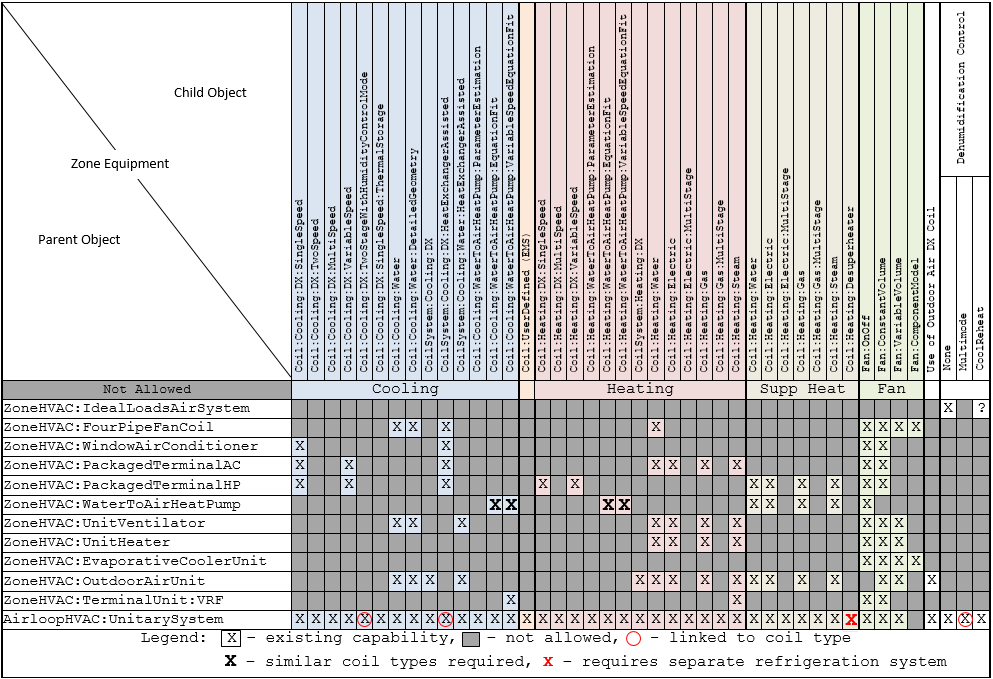
\includegraphics{media/ZoneComponentMatrix.png}
\caption{}
\end{figure}

\subsection{ZoneHVAC:EquipmentList}\label{zonehvacequipmentlist}

The first list encountered in the \hyperref[zonehvacequipmentconnections]{ZoneHVAC:EquipmentConnections} statement is the ZoneHVAC:EquipmentList. This object lists all HVAC equipment serving the zone. Each item in the list has four fields associated with it: Object Type, Name, Cooling Sequence and Heating or No-Load Sequence The Object Type and Name identify the specific equipment object. Cooling Sequence and Heating or No-Load Sequence specify the order of simulation for zones with more than one type of HVAC equipment.

Note that a \hyperref[zonehvacairdistributionunit]{ZoneHVAC:AirDistributionUnit} must be listed in this statement if there is a forced air system serving the zone from an air loop.

\subsubsection{Inputs}\label{inputs-2-048}

\paragraph{Field: Name}\label{field-name-1-050}

Unique identifying name.

\paragraph{Field: Load Distribution Scheme}

The Load Distribution Scheme selects the algorithm used to allocate the current zone load across the zone equipment. There are four choices: SequentialLoad, UniformLoad, UniformPLR, and SequentialUniformPLR. The default is SequentialLoad. In all cases, the equipment operates in the order specifed by the Zone Equipment Cooling Sequence and Heating or No-Load Sequence fields.

\begin{itemize}
\item
  SequentialLoad loads each piece of available equipment sequentially with the full remaining load.
\item
  UniformLoad evenly distributes the total load equally among all available components on the equipment list for the current load type.
\item
  UniformPLR evenly distributes the total load among all available components on the equipment list for the current load type at a uniform part load ratio (PLR).
\item
  SequentialUniformPLR determines how many of the available components are required to meet the current load, then distributes the load at a uniform part load ratio (PLR).
\end{itemize}
\paragraph{Field Set (Zone Equipment: Object Type, Name, Cooling Sequence, Heating or No-Load Sequence, Sequential Cooling Fraction Schedule, Sequential Heating Fraction Schedule)}\label{field-set-zone-equipment-object-type-name-cooling-sequence-heating-or-no-load-sequence}

This set is used together in order to sequence the equipment for heating and cooling. The \#1 sequence equipment will try to meet the entire demand with its capacity and then pass the results on to the \#2 and so on for both heating and cooling. This object is extensible, so additional groups of the following four fields can be added to the end of this object.

Equipment is simulated in the order specified by Zone Equipment Cooling Sequence and Zone Equipment Heating or No-Load Sequence, depending on the current thermostat request. For equipment of similar type, assign sequence 1 to the first system intended to serve that type of load, assign sequence 2 to the next system, and so on. For situations where one or more equipment types has limited capacity or limited control capability, order the sequence so that the most controllable piece of equipment runs last. For example, with a dedicated outdoor air system (DOAS), the air terminal for the DOAS should be assigned Heating Sequence = 1 and Cooling Sequence = 1. Any other equipment should be assigned sequence 2 or higher so that it will see the net load after the DOAS air is added to the zone.

\paragraph{Field: Zone Equipment \textless{}x\textgreater{} Object Type}\label{field-zone-equipment-x-object-type}

Type of zone equipment such as air distribution unit, baseboard, window air conditioner, etc. The current legal types are listed in the following table:

% table 27
\begin{longtable}[c]{@{}l@{}}
\caption{Legal Zone Equipment Types (ZoneHVAC:EquipmentList) \label{table:legal-zone-equipment-types-zonehvac}} \tabularnewline
\toprule
Legal Zone Equipment Types \tabularnewline
\midrule
\endfirsthead

\caption[]{Legal Zone Equipment Types (ZoneHVAC:EquipmentList)} \tabularnewline
\toprule
Legal Zone Equipment Types \tabularnewline
\midrule
\endhead

Fan:ZoneExhaust \tabularnewline
WaterHeater:HeatPump:PumpedCondenser \tabularnewline
WaterHeater:HeatPump:WrappedCondenser \tabularnewline
ZoneHVAC:AirDistributionUnit \tabularnewline
ZoneHVAC:Baseboard:Convective:Electric \tabularnewline
ZoneHVAC:Baseboard:Convective:Water \tabularnewline
ZoneHVAC:Baseboard:RadiantConvective:Electric \tabularnewline
ZoneHVAC:Baseboard:RadiantConvective:Water \tabularnewline
ZoneHVAC:Baseboard:RadiantConvective:Steam \tabularnewline
ZoneHVAC:Dehumidifier:DX \tabularnewline
ZoneHVAC:EnergyRecoveryVentilator \tabularnewline
ZoneHVAC:FourPipeFanCoil \tabularnewline
ZoneHVAC:HighTemperatureRadiant \tabularnewline
ZoneHVAC:IdealLoadsAirSystem \tabularnewline
ZoneHVAC:LowTemperatureRadiant:ConstantFlow \tabularnewline
ZoneHVAC:LowTemperatureRadiant:Electric \tabularnewline
ZoneHVAC:LowTemperatureRadiant:VariableFlow \tabularnewline
ZoneHVAC:OutdoorAirUnit \tabularnewline
ZoneHVAC:PackagedTerminalAirConditioner \tabularnewline
ZoneHVAC:PackagedTerminalHeatPump \tabularnewline
ZoneHVAC:RefrigerationChillerSet \tabularnewline
ZoneHVAC:UnitHeater \tabularnewline
ZoneHVAC:UnitVentilator \tabularnewline
ZoneHVAC:WindowAirConditioner \tabularnewline
ZoneHVAC:WaterToAirHeatPump \tabularnewline
ZoneHVAC:VentilatedSlab \tabularnewline
\bottomrule
\end{longtable}

\paragraph{Field: Zone Equipment \textless{}x\textgreater{} Name}\label{field-zone-equipment-x-name}

Name of the zone equipment used in the object definition of its type.

\paragraph{Field: Zone Equipment \textless{}x\textgreater{} Cooling Sequence}\label{field-zone-equipment-x-cooling-sequence}

Specifies the zone equipment simulation order when the zone thermostat requests cooling.

\paragraph{Field: Zone Equipment \textless{}x\textgreater{} Heating or No-Load Sequence}\label{field-zone-equipment-x-heating-or-no-load-sequence}

Specifies the zone equipment simulation order when the zone thermostat requests heating or no load.

\paragraph{Field: Zone Equipment \textless{}x\textgreater{} Sequential Cooling Fraction Schedule Name}\label{field-zone-equipment-x-sequential-cooling-fraction}

References a schedule that specifies the fraction of the remaining cooling load this equipment will attempt to serve. Only applies if the load distribution scheme is SequentialLoad. Leaving this blank indicates a constant schedule of 1.0.

\paragraph{Field: Zone Equipment \textless{}x\textgreater{} Sequential Heating Fraction Schedule Name}\label{field-zone-equipment-x-sequential-heating-fraction}

References a schedule that specifies the fraction of the remaining heating load this equipment will attempt to serve. Only applies if the load distribution scheme is SequentialLoad. Leaving this blank indicates a constant schedule of 1.0.

Examples of this statement in an IDF are:

\begin{lstlisting}

    ZoneHVAC:EquipmentList,
      Zone1Equipment,                !- Name
      SequentialLoad,                !- Load Distribution Scheme
      ZoneHVAC:AirDistributionUnit,  !- Zone Equipment 1 Object Type
      Zone1TermReheat,               !- Zone Equipment 1 Name
      1,                             !- Zone Equipment 1 Cooling Sequence
      1,                             !- Zone Equipment 1 Heating or No-Load Sequence
      ,                              !- Zone Equipment 1 Sequential Cooling Fraction Schedule Name
      ;                              !- Zone Equipment 1 Sequential Heating Fraction Schedule Name


    ZoneHVAC:EquipmentList,
      Zone1Equipment,                !- Name
      SequentialLoad,                !- Load Distribution Scheme
      ZoneHVAC:AirDistributionUnit,  !- Zone Equipment 1 Object Type
      Zone1TermReheat,               !- Zone Equipment 1 Name
      1,                             !- Zone Equipment 1 Cooling Sequence
      1,                             !- Zone Equipment 1 Heating or No-Load Sequence
      0.5,                           !- Zone Equipment 1 Sequential Cooling Fraction
      0.5,                           !- Zone Equipment 1 Sequential Heating Fraction
      ZoneHVAC:WaterToAirHeatPump,   !- Zone Equipment 2 Object Type
      Zone1WTAHP,                    !- Zone Equipment 2 Name
      2,                             !- Zone Equipment 2 Cooling Sequence
      2,                             !- Zone Equipment 2 Heating or No-Load Sequence
      0.5,                           !- Zone Equipment 2 Sequential Cooling Fraction
      0.5;                           !- Zone Equipment 2 Sequential Heating Fraction
\end{lstlisting}
